\chapter[Beyond RL for Real World Robotic Navigation]{Beyond Reinforcement Learning for Real World Robotic Visual Navigation}\label{ch:beyond-rl}

\lettrine{\textcolor{accent_color}{W}}{hen} it comes to training robots to navigate in the real world, \acrshort{rl} has been the go-to approach for many years.
However, \acrshort{rl} has its limitations, especially when it comes to real-world applications.
Using online \acrshort{rl} algorithms requires querying environments to learn.
This is a problem because querying real environments is expensive and time-consuming, and querying simulated environments is not always a good proxy for real-world performance.

Furthermore, another limitation of online \acrshort{rl} is that it requires a large number of interactions to learn.
This is known as sample-inefficiency, and it is a major bottleneck for real-world applications, as it requires a lot of time and resources to collect enough interactions to train a robot.
In this chapter, two alternative approaches to \acrshort{rl} for robotic visual navigation are explored: Offline Reinforcement Learning and \acrfull{mil}.


\section{Offline Reinforcement Learning for Robotic Visual Navigation}\label{sec:offline_rl4rvsn}

The first approach that is explored is Offline \acrshort{rl}~\cite{levine2020}.
Offline \acrshort{rl} consists of learning policies from a fixed dataset consisting of human demonstrations and their associated reward signals.
This can be a powerful approach for training agents in complex environments, as it allows the agent to learn from a large amount of data without the need to interact with the environment.
Therefore, in this section, a novel approach to train \acrshort{vsn} agents without ever querying an environment is proposed, by leveraging on the Offline \acrshort{rl} paradigm.
This approach is called \textbf{Off}line Visual Semantic \textbf{Nav}igation (OffNav).

Technically, an \acrfull{iql}~\cite{kostrikov2022offline} offline \acrshort{rl} algorithm is implemented using the decentralized distributed philosophy of \acrshort{ddppo}~\cite{wijmans2020} to create DD-\acrshort{iql}, a decentralized distributed version of \acrshort{iql}\@.
The DD-\acrshort{iql} is trained against a fixed dataset containing thousands of human navigation experiences~\cite{ramrakhya2023}.
As depicted in Figure~\ref{fig:abstract_offnav}, the OffNav approach is proposed, capable of efficiently learning the navigation policy required by a \acrshort{vsn} agent from human demonstrations.
Subsequently, these policies can be deployed across various scenarios, and if necessary, further refined through online \acrshort{rl} for more specific tasks.

To demonstrate the capabilities of this implementation, a small analysis of its performance using different environments from HM3D dataset~\cite{Ramakrishnan2021HabitatMatterport3D} is carried out.
Preliminary results show that the DD-\acrshort{iql} implementation is able to learn navigation policies effectively.
To the best of the author's knowledge, this is the first time that an offline \acrshort{rl} algorithm is implemented for \acrshort{vsn}\@ and large environments, predicting actions directly from raw input observations.

\begin{figure}
    \centering
    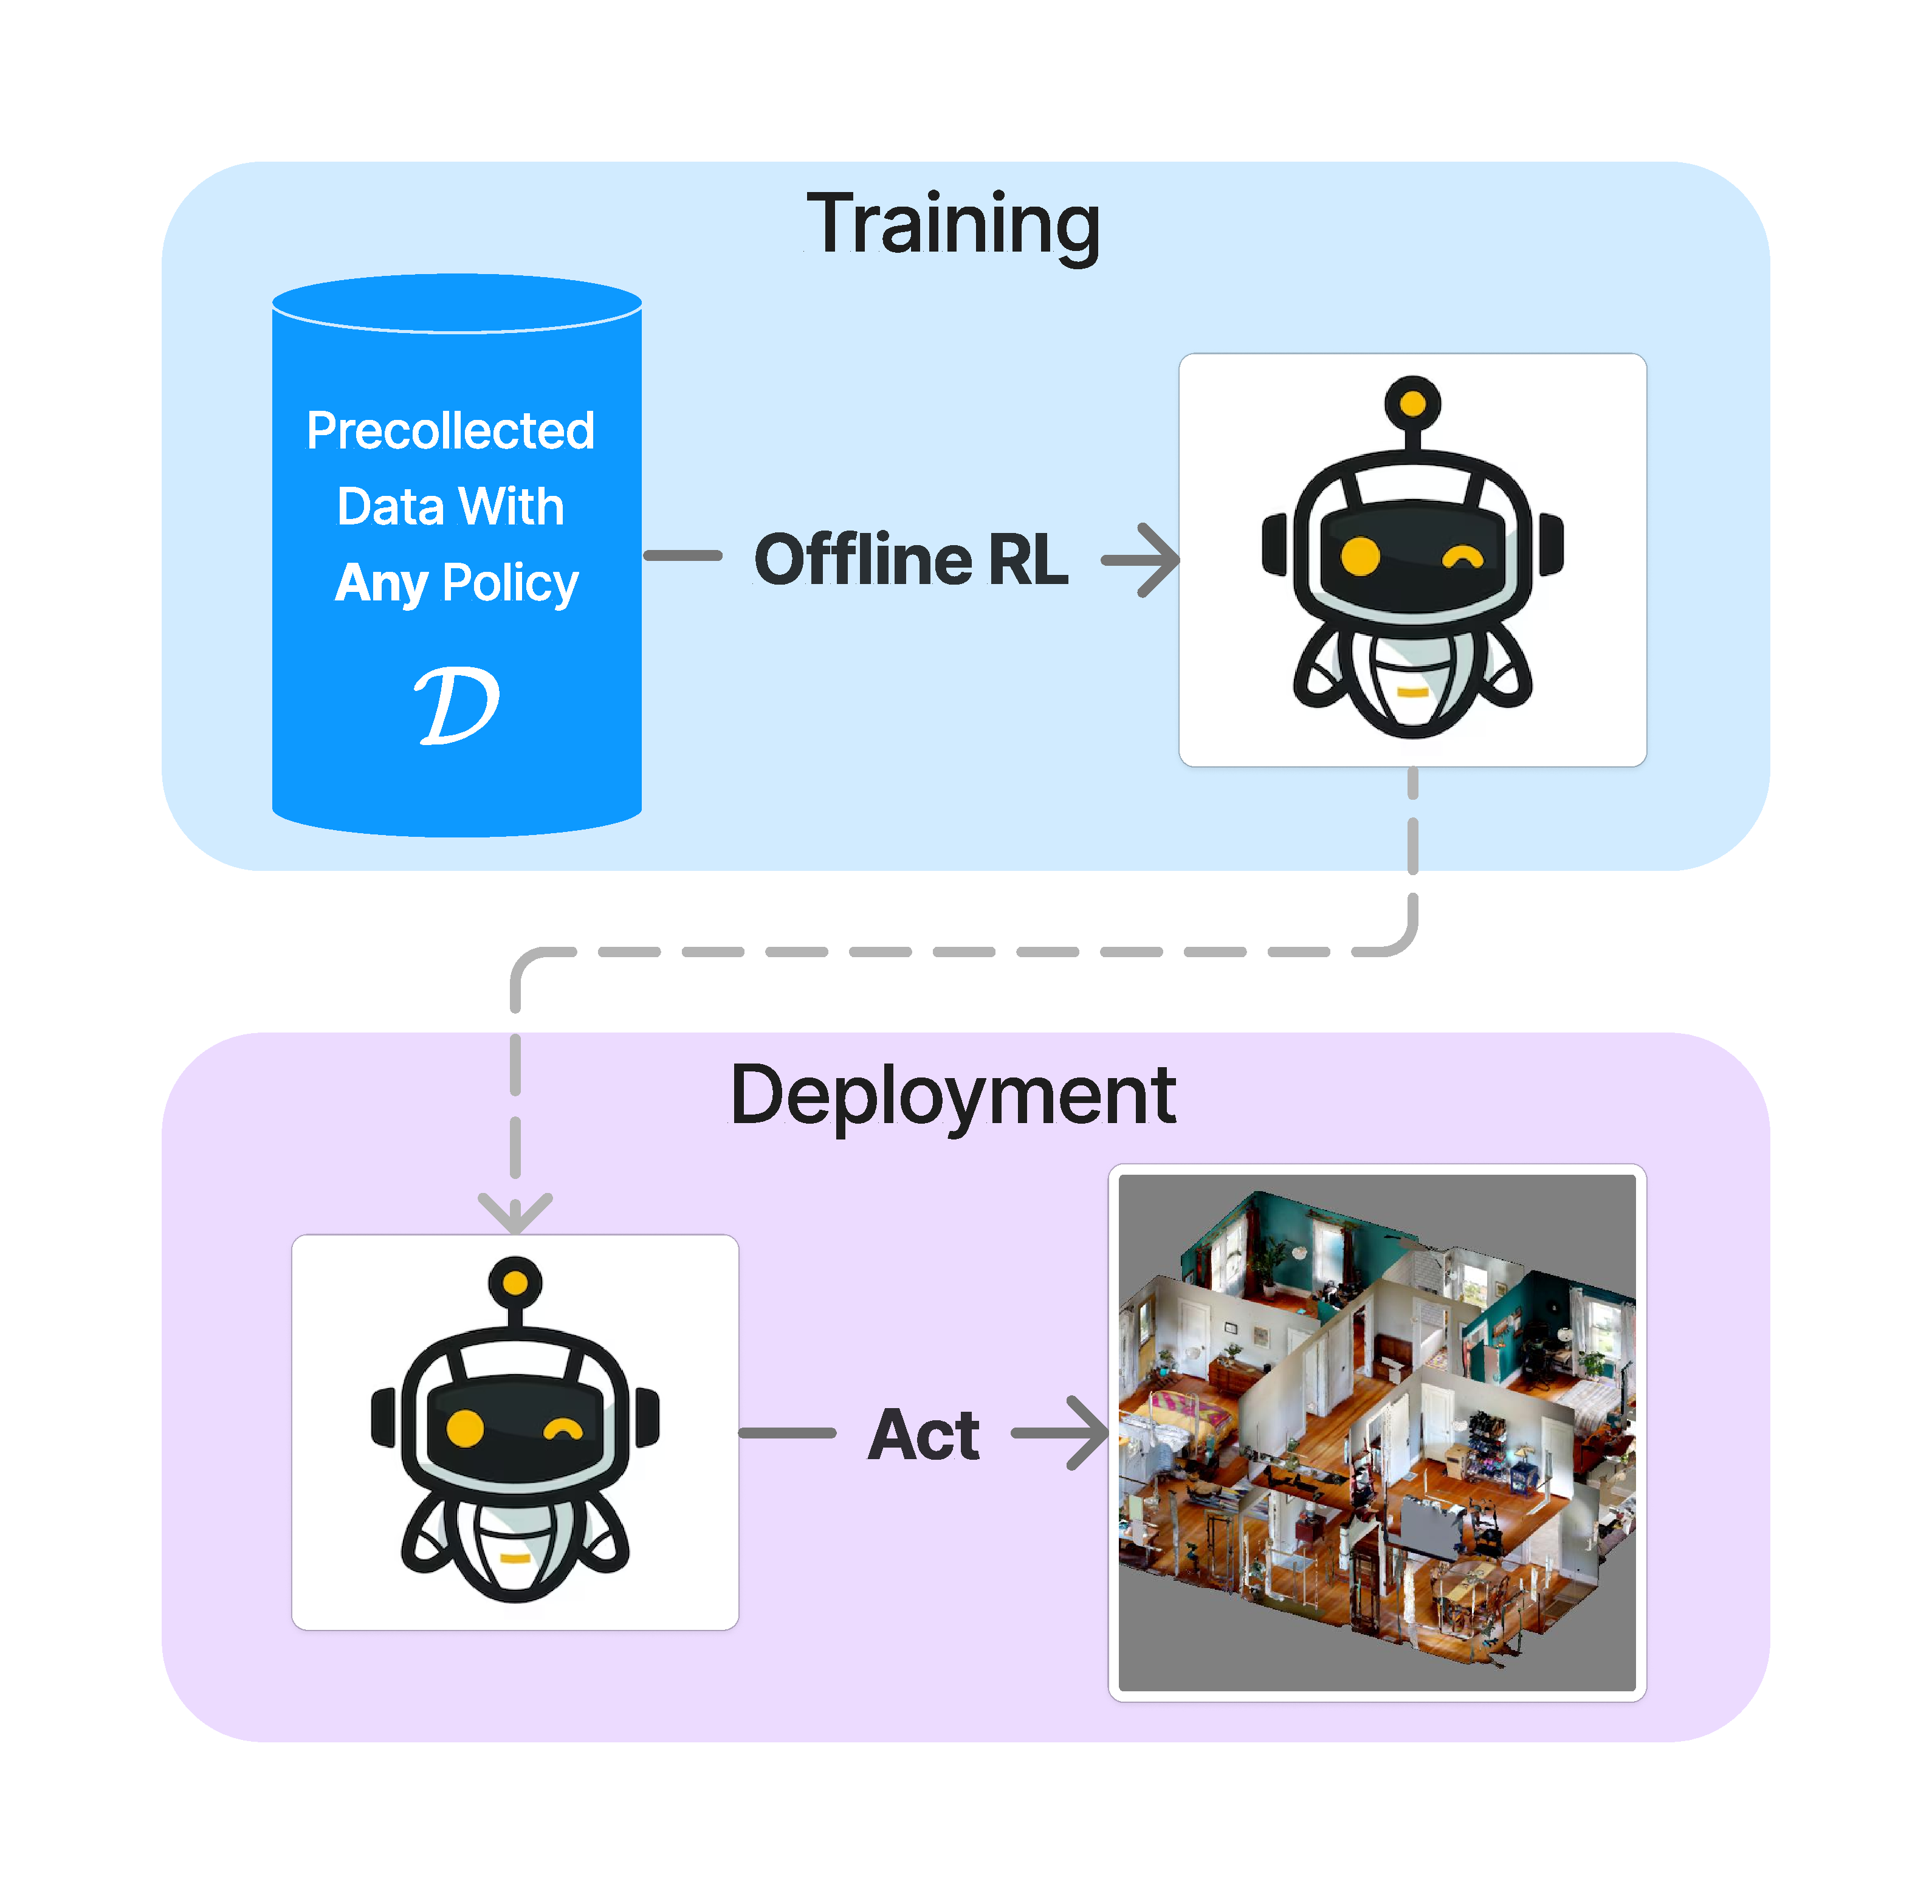
\includegraphics[width=0.7\linewidth]{figures/offnav/graphical_abstract}
    \caption[Offline RL diagram]{
        By leveraging on the offline reinforcement learning paradigm, agents can be trained from a fixed dataset of navigation experience, without querying any environment.
        This opens the possibility to create many navigation datasets from any navigation agent in any \textbf{real or simulated} environment, and then use them to train new agents for different scenarios without the need to ever query that environment.
    }
    \label{fig:abstract_offnav}
\end{figure}

\subsection{Offline Visual Semantic Navigation}\label{subsec:offline-navigation}

In this section, \acrshort{objnav} navigation~\cite{batra2020} is studied, a setup in which an agent is asked to navigate to a target object in an environment.
To perform this task, the agent does it using only egocentric perceptions.
Specifically, the agent receives RGB images and GPS+Compass information that provides the agent with the current position and orientation relative to the starting point.
The set of movements is discrete and consists of the following actions: \turnleft, \turnright, \moveforward, \lookup, \lookdown, and \stopac.
If the agent samples the \stopac action within 1 m Euclidean distance with respect to the target object within a 500-step time limit, the episode is considered successful.
In the other case, it is considered a failure.
The performance of the navigation is measured by averaging the success over all the episodes present in an evaluation, and it receives the name of \acrfull{sr}.
The \acrfull{spl} metric is also reported, which is the success rate weighted by the ratio between ideal and actual path length.

Since an offline \acrshort{rl} setup is used, a previously collected dataset of navigation experience is needed.
The dataset that was chosen is collected in~\cite{ramrakhya2023}.
It consists of 77k episodes of human navigation trajectories using the HM3D~\cite{Ramakrishnan2021HabitatMatterport3D} dataset.

The policies are trained using the DD-\acrshort{iql} implementation on the human demonstrations.
The objetive is to find a policy with optimal parameters $\phi^*$ that maximizes the expected return from the dataset.
To do so, the \acrshort{iql} algorithm relies on the use of expectile regression to modify a \acrfull{td} loss.
This modified \acrshort{td} loss is able to learn an approximate Q-function from the dataset actions.
This Q-function does not explicitly represent the corresponding policy, so a separate policy extraction step is needed.
For policy extraction, advantage-weighted regression~\cite{peters2007, peng2019advantageweighted} is used:

\begin{equation}
    L_\pi(\phi)=\mathbb{E}_{(s, a) \sim \mathcal{D}}\left[\exp \left(\beta\left(Q_{\hat{\theta}}(s, a)-V_\psi(s)\right)\right) \log \pi_\phi(a|s)\right]\; ,
    \label{eq:loss}
\end{equation}

where $\beta \in [0, \infty)$ controls the trade-off between cloning the expert policy and maximizing the Q-function.
This loss can be seen as a selection of the most optimal actions to clone in the dataset.
Inflection weighting~\cite{wijmans2019} is also employed to modify the loss function, thereby giving more importance to those time steps where there is a change in actions.

For the policy architecture, a simple \acrshort{cnn}+\acrshort{rnn} model from\cite{ramrakhya2023} is used.
The difference is that ResNet18 is used for the visual encoders.
The same architecture is copied for the policy net, the Q net, and the Q target net.
For the V net, only the visual encoder and a single linear layer are used, without any recurrent module.

\subsection{Experiments and Results}\label{subsec:experiments_offnav}

Is an offline \acrshort{rl} algorithm able to learn navigation policies effectively?
To answer this question, the DD-\acrshort{iql} model is trained using the expert demonstrations on five different experimental setups.
These setups have been designed with an incremental difficulty.
The first three are evaluated in the same environments in which the agents were trained, while the last two are evaluated in different environments.
The details of the setups are depicted on figure~\ref{fig:setups}.

The results are compared with the current state-of-the-art model PirlNav~\cite{ramrakhya2023}.
This model is based on a two-phase training schedule.
The first phase is a supervised learning phase, where the model is trained using behavior cloning on the expert demonstrations.
The second phase is a reinforcement learning phase, where the model is fine-tuned using \acrshort{ddppo}~algorithm~\cite{wijmans2020}.
For a fair comparison, the PirlNav agent is trained using only the behavior cloning phase on the same setups as the OffNav model.

Results are shown on table~\ref{tab:success}.
It can be seen that both methods obtain similar performance on setups 1 to 3.
Offnav method outperforms PirlNav on setup 2, while PirlNav outperforms OffNav on setup 3, and both of them obtain 100 \% \acrshort{sr} on setup 1.
When evaluated on setup 4, PirlNav outperforms OffNav by 2.27\% absolute points.
However, on setup 5, the most challenging one, OffNav outperforms PirlNav by 8.69\% absolute points.

\begin{table}
    \centering
    \begin{tabular}{c|ccc}
        \toprule
        \textit{Experimental Setup} & \textit{OffNav}  & \textit{PirlNav} \\
        \midrule
        \textsc{Setup 1}            & 100\%            & 100\%            \\
        \textsc{Setup 2}            & \textbf{79.31\%} & 72.50\%          \\
        \textsc{Setup 3}            & 75.78\%          & \textbf{77.63\%} \\
        \textsc{Setup 4}            & 25.00\%          & \textbf{27.27\%} \\
        \textsc{Setup 5}            & \textbf{34.78\%} & 26.09\%          \\
        \bottomrule
    \end{tabular}
    \caption{Success Rate for OffNav and PirlNav methods on the five experimental setups.}
    \label{tab:success}
\end{table}

\begin{figure}
    \centering
    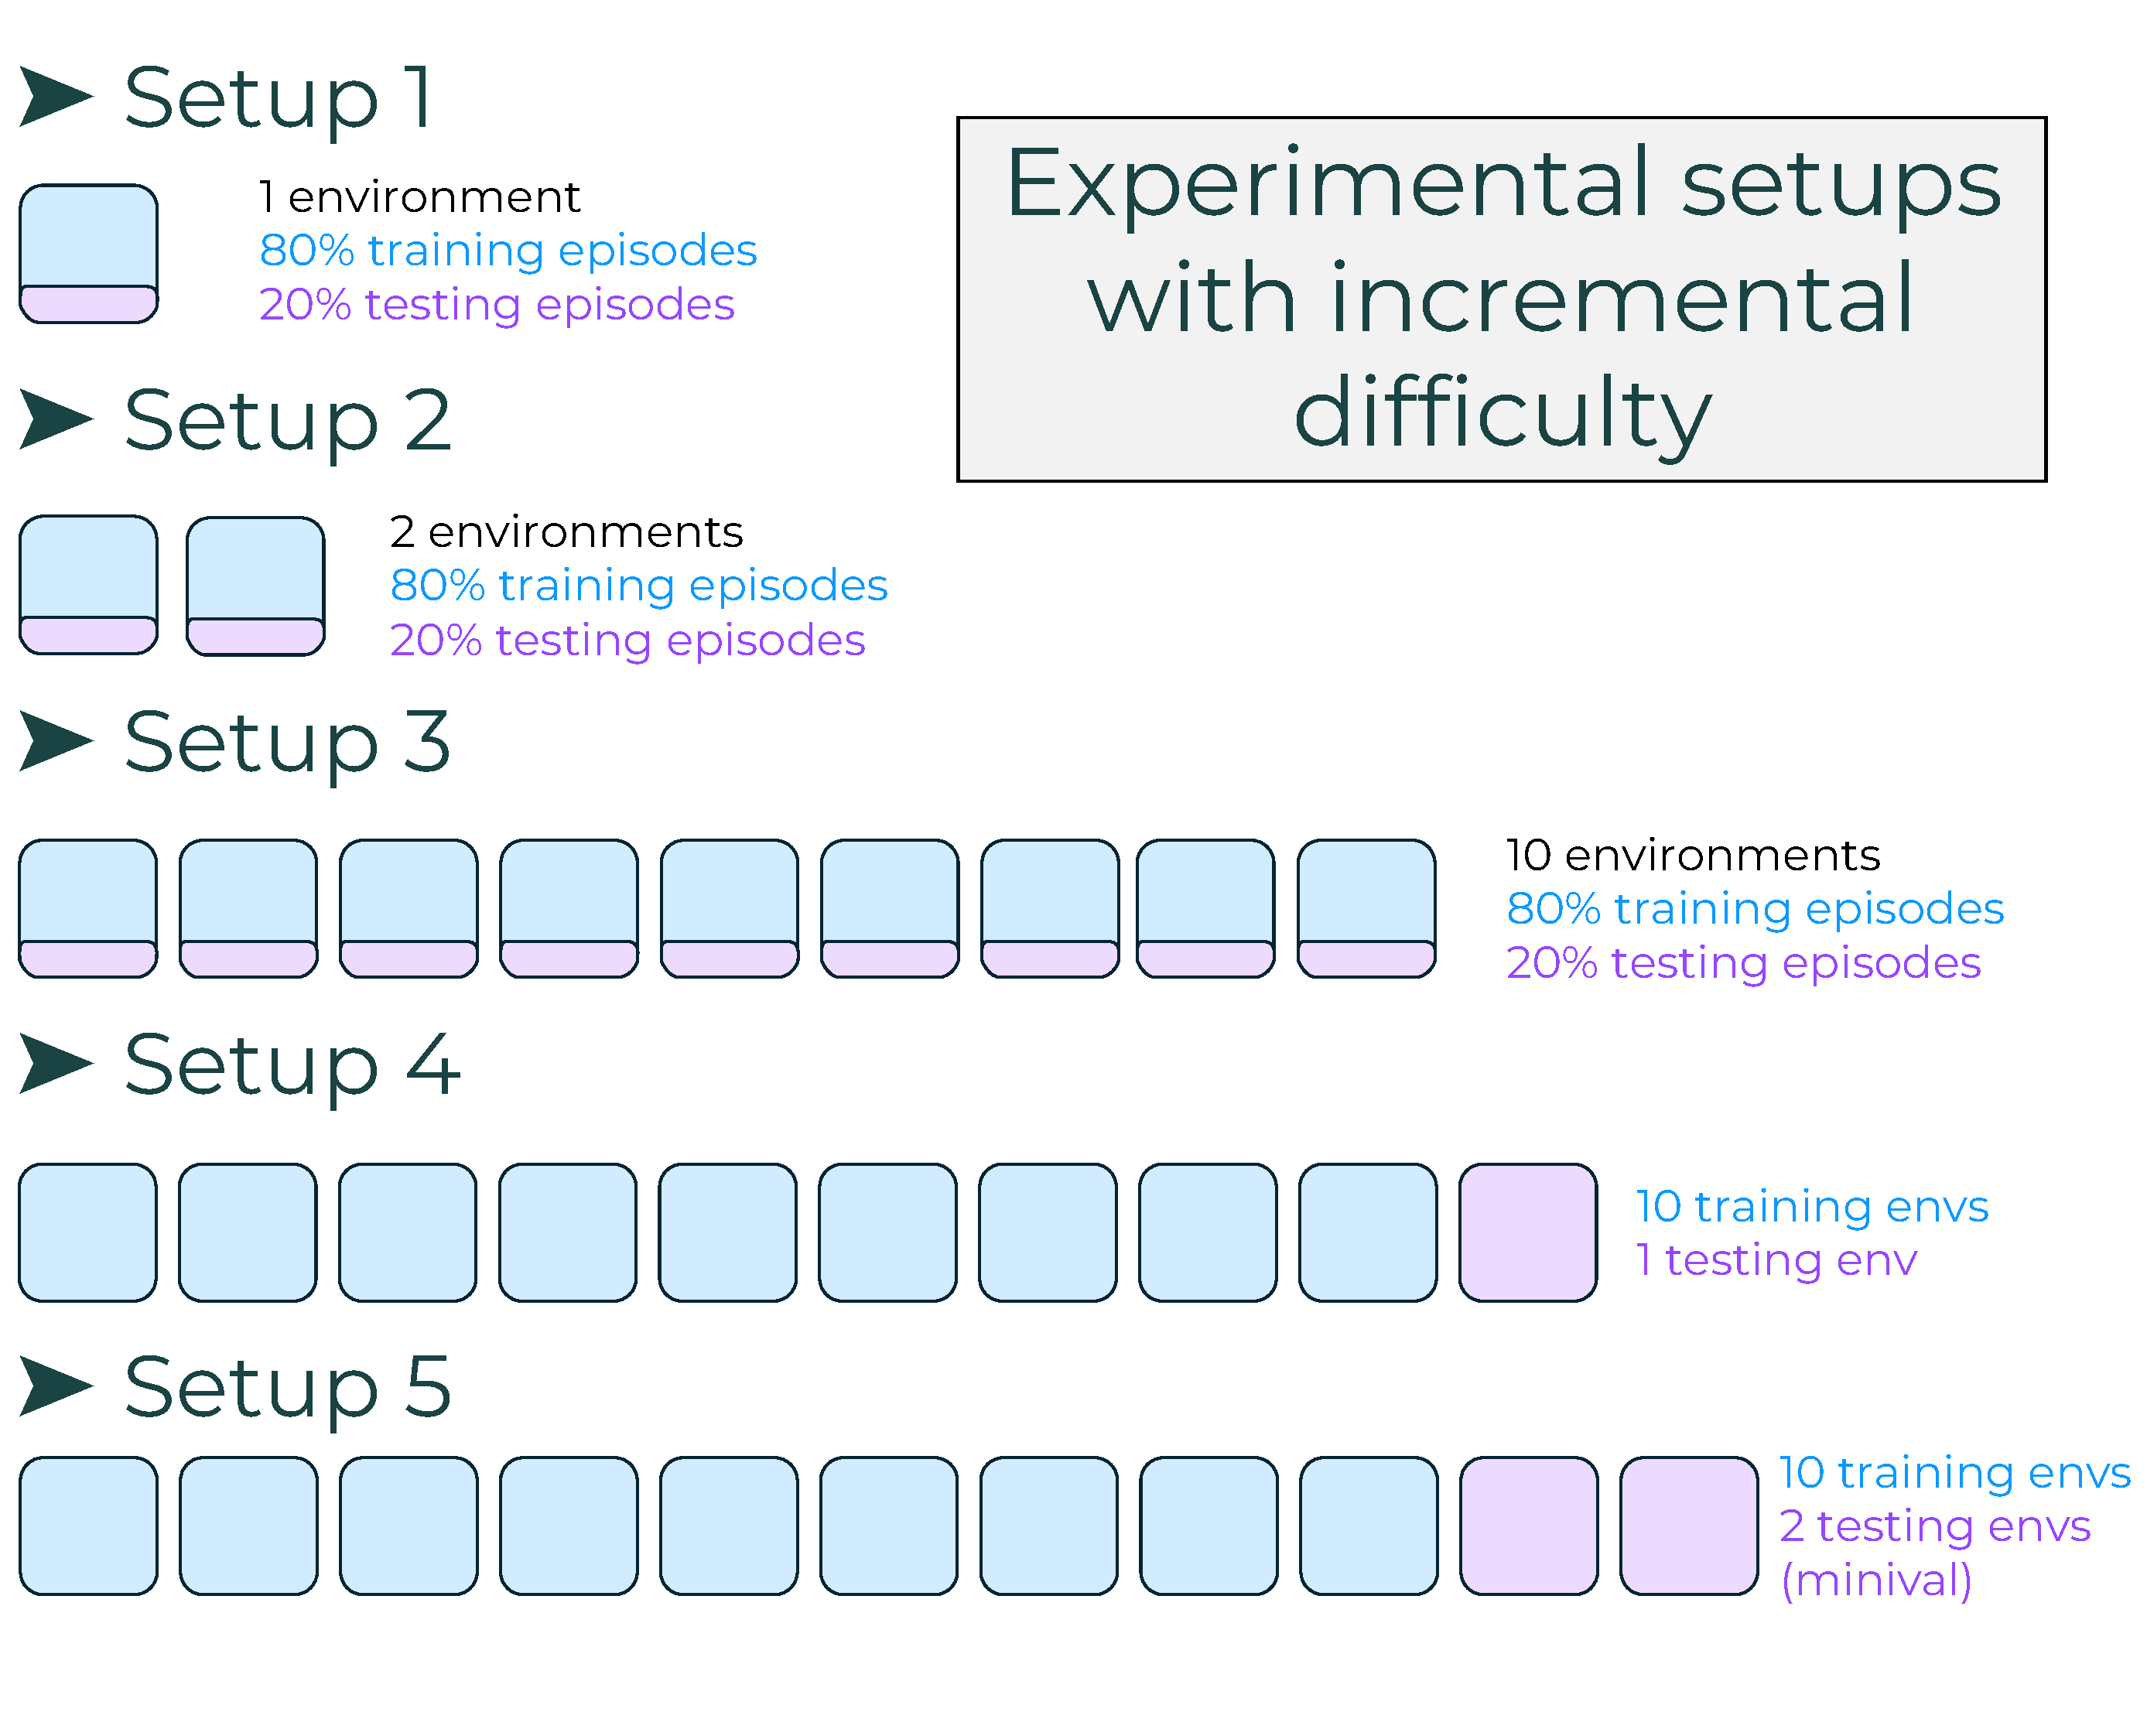
\includegraphics[width=0.8\linewidth]{figures/offnav/experimental_setups}
    \caption{Five experimental setups designed with an incremental difficulty.}
    \label{fig:setups}
\end{figure}

\subsection{Conclusions and Future Work}\label{subsec:conclusions_offnav}

From the results obtained in the experiments, it can be concluded that the proposed OffNav method is able to learn navigation policies effectively from human demonstrations.
It can also be seen that the method is able to generalize to unseen environments, as shown in setups 4 and 5, and outperform the state-of-the-art model PirlNav~\cite{ramrakhya2023} in the most challenging one.
Future work will focus on training the policy with more diverse environments to improve its generalization capabilities and further extend this analysis.
The next section explores a different approach to training agents from a fixed dataset, but with the ability to adapt quickly to new tasks with few examples.


\section{Meta Imitation Learning for Real World Navigation}\label{sec:mil-for-real-world-navigation}

In section~\ref{sec:offline_rl4rvsn}, the possibility of training agents from a fixed dataset of human demonstrations using offline reinforcement learning was explored.
Despite the elimination of the need to query environments, this approach still requires a large amount of data to learn effectively.
This reduces the applicability of this approach in real-world scenarios, where collecting large datasets can become an unfeasible task.
To address this issue, a different approach that can also learn from a fixed dataset, but with the ability to adapt quickly to new tasks with few examples is explored.
This will help to bridge the gab between training agents in simulation and deploying them in the real world.

This second approach that is explored is known as Meta Imitation Learning~\cite{finnOneShotVisualImitation2017}.
Here a combination of two different paradigms is used: Imitation Learning and Meta Reinforcement Learning.
On the one hand, Meta Reinforcement learning~\cite{Beck_2025} is a set of techniques that try to teach agents to learn how to learn, enabling them to adapt quickly to new tasks with few examples.
Imitation Learning~\cite{10602544}, on the other hand, is a paradigm that allows agents to learn from demonstrations provided by an expert.
Thus, \acrfull{mil} is a combination of both realms, allowing agents to learn from a small number of demonstrations and adapt quickly to new tasks.
This approach can be described as a meta-learning algorithm that learns to imitation learn.
Figure~\ref{fig:abstract_metanav} illustrates the proposed approach, which is called \textbf{Meta} Visual Semantic \textbf{Nav}igation (MetaNav).
In this setting, a parametrized policy $\pi_\phi$ is learned that can adapt to new tasks by learning from a small number of gradient updates.
Due to this adaptability, the policy can be trained on simulation using a set of task demonstrations and then deployed in the real world to perform new tasks.

The main question sought to be answered is: \textit{Can visual navigation policies be learned via meta-imitation learning that can adapt to new tasks with few examples?}
To answer this question, a meta-imitation learning algorithm based on the work of~\cite{finnOneShotVisualImitation2017} is implemented.
The algorithm is trained on a small set of different environments from HM3D dataset~\cite{Ramakrishnan2021HabitatMatterport3D}.
Preliminary results show that the algorithm is able to learn visual navigation policies that can adapt to new tasks with few examples.
To the best of the author's knowledge, this is the first time that a meta-imitation learning algorithm is implemented for \acrshort{vsn}\@ and large environments, predicting actions directly from raw input observations.

\begin{figure}
    \centering
    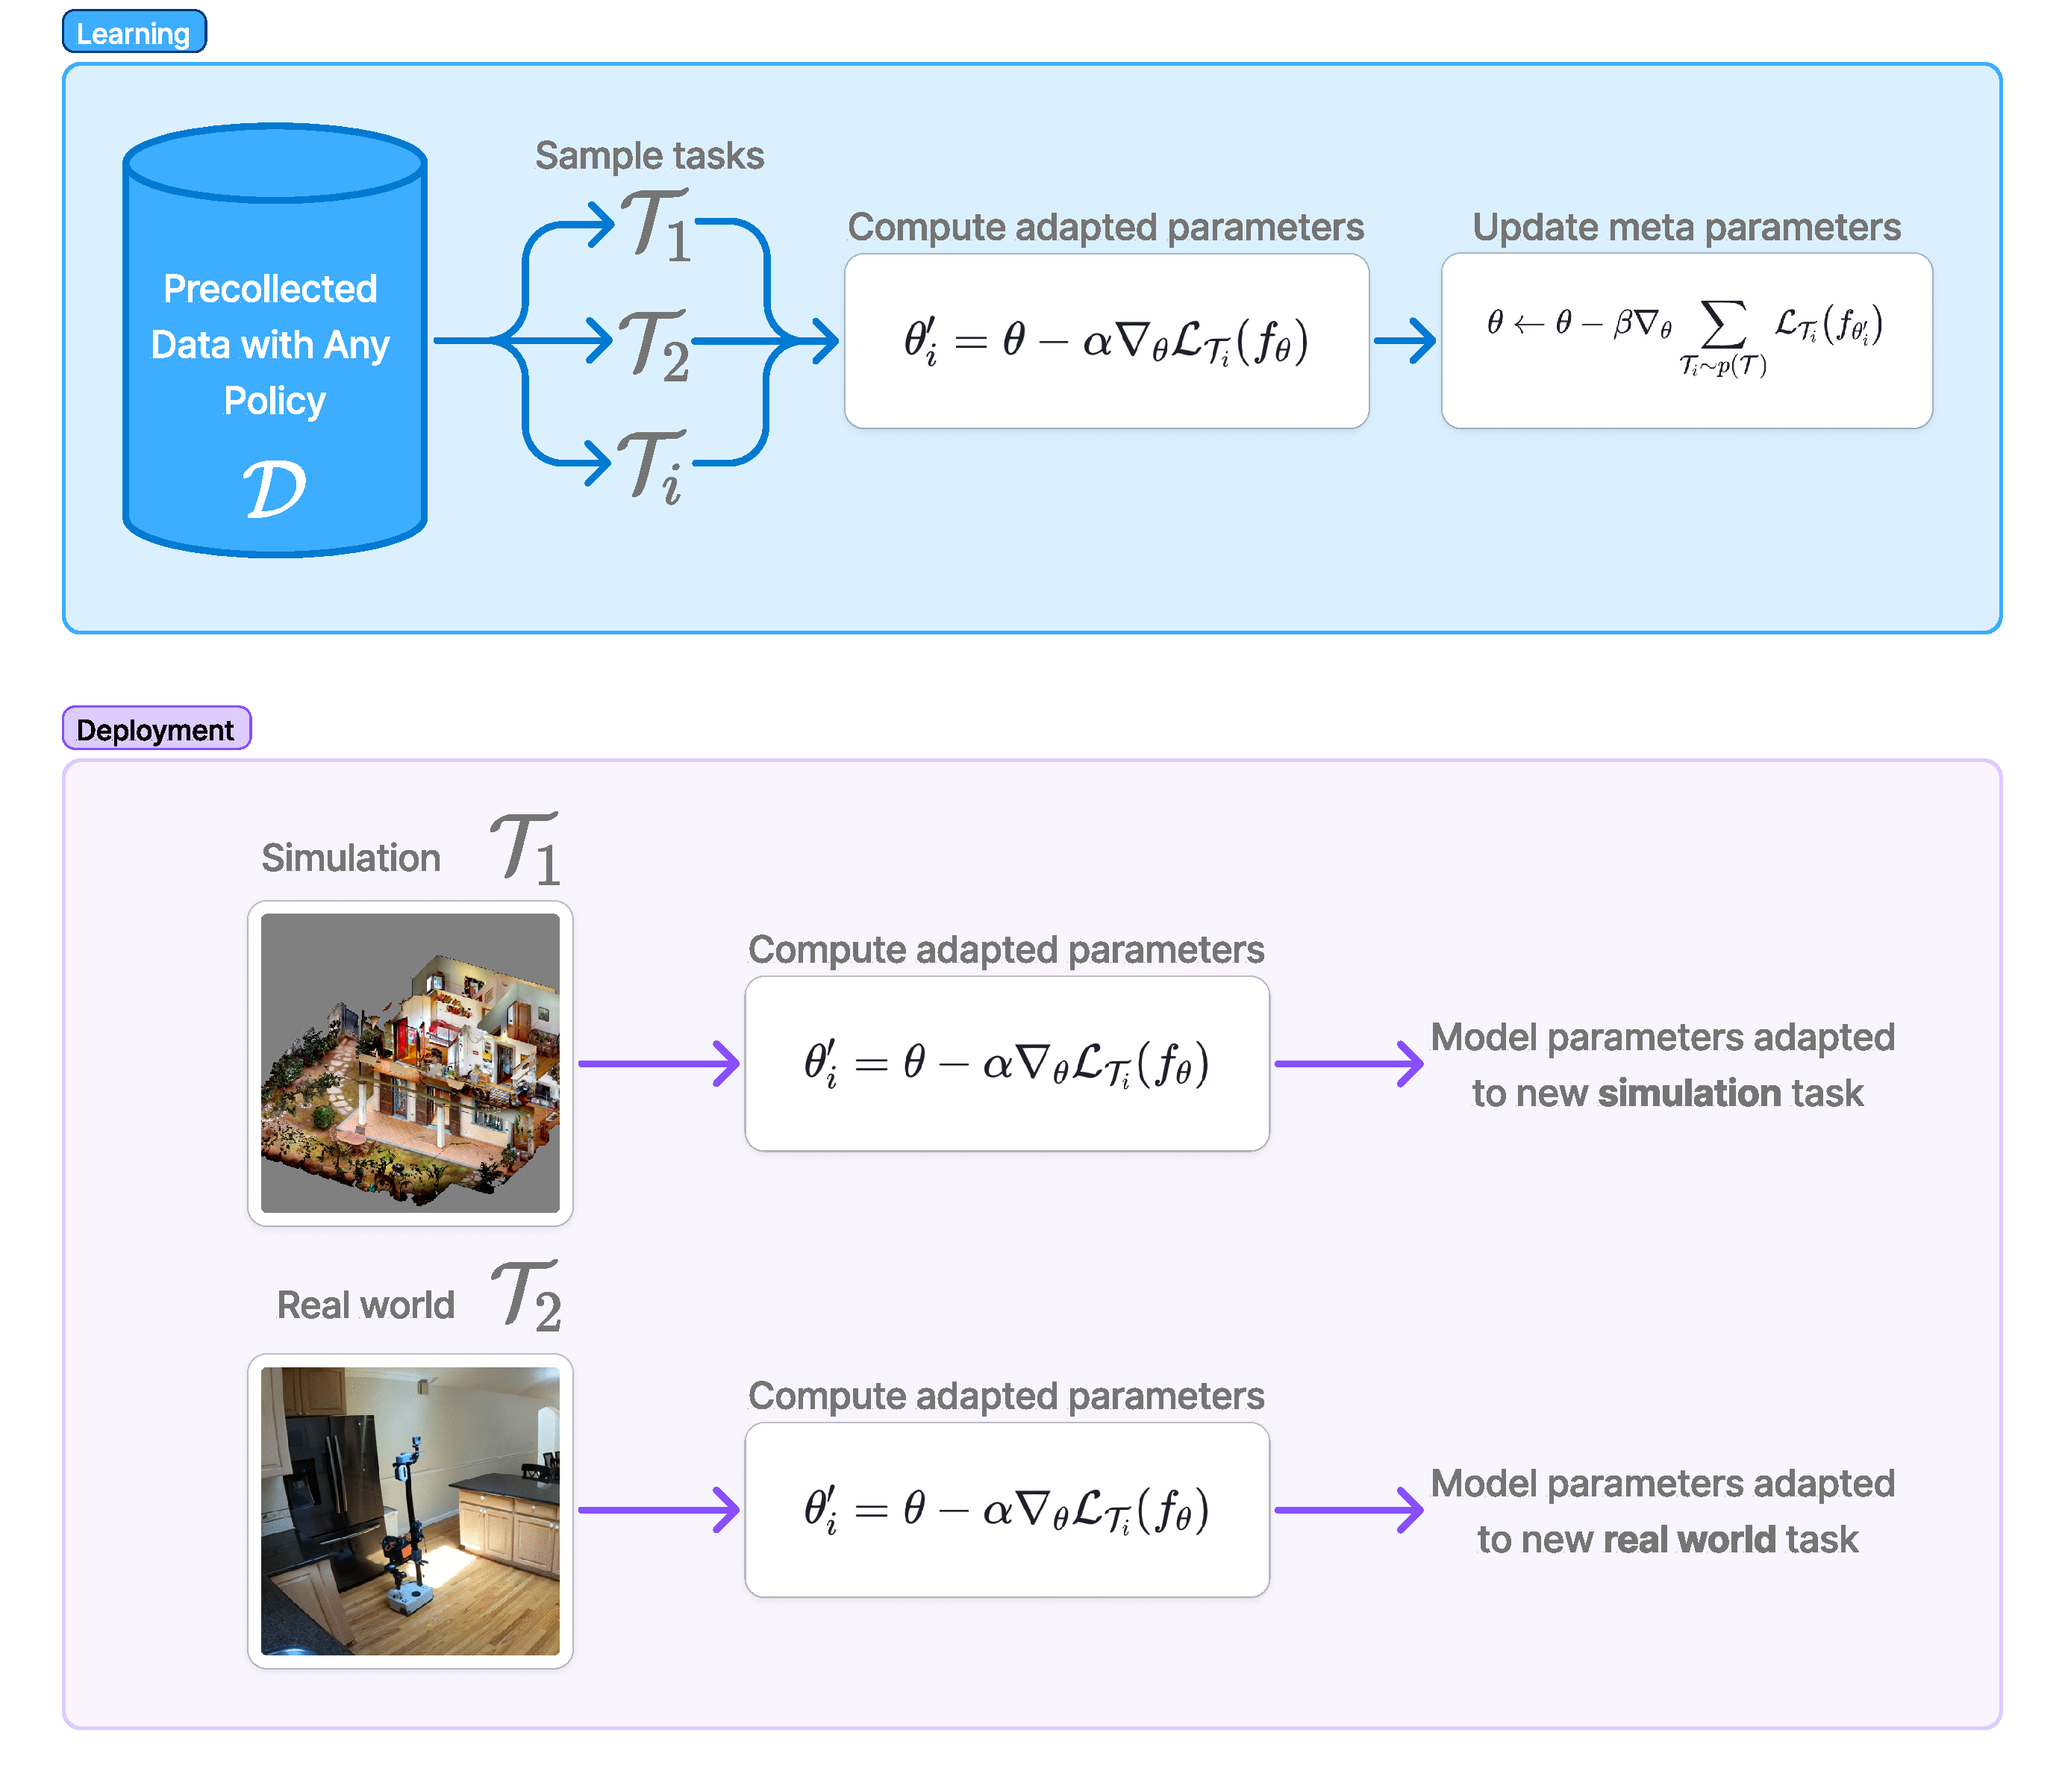
\includegraphics[width=0.7\linewidth]{figures/metanav/graphical_abstract}
    \caption[Meta-imitation learning diagram]{
        The meta-imitation learning approach transforms the usual learning problem into a collection of small similar problems called tasks.
        Here, the goal is to learn a policy that is generally good on all of them, while also adapting quickly to new tasks by using a small amount of new experience.
    }
    \label{fig:abstract_metanav}
\end{figure}

\subsection{Meta-Imitation Learning for Robotic Visual Navigation}\label{subsec:meta-imitation-learning-for-robotic-visual-navigation}

In this section, the proposed Meta Imitation Learning algorithm for robotic visual navigation is described.
The approach of~\cite{finnOneShotVisualImitation2017} is followed, in which a vision-based policy is trained to adapt to new tasks with few examples.

\subsubsection{Problem setting}\label{subsubsec:problem-setting}

As described in section~\ref{subsec:offline-navigation}, the focus is on \acrshort{objnav} navigation~\cite{batra2020}, where an agent must reach a specified target object within an environment by sampling actions from a discrete set.
The available actions are discrete and include: \turnleft, \turnright, \moveforward, \lookup, \lookdown, and \stopac.
An episode is considered successful if the agent selects the \stopac action within 1 meter of the target object and within a 500-step limit; otherwise, it is deemed a failure.
The agent relies solely on egocentric observations to accomplish this task.
In particular, it receives RGB images and GPS+Compass data, which provide its current position and orientation relative to the starting point.

Since an imitation learning setup is used, a previously collected dataset of navigation experience is needed.
The dataset that was chosen is collected in~\cite{ramrakhya2023}.
It consists of 77k episodes of human navigation trajectories using the HM3D~\cite{Ramakrishnan2021HabitatMatterport3D} dataset.
This dataset consists of a set of photorealistic 3D indoor environments, each containing a variety of objects and different scenes.

Finally, a task is defined as a tuple of the form $\mathcal{T} = (G, S)$, where $G$ is the target object and $S$ the scene in which the navigation is taking place.
Each task can contain multiple demonstrations $\tau_i$, each of them recorded by a human and always on the same scene and seeking the same target object.
The variability of the demonstrations comes from the random starting points in each episode and the different paths that the human can take to reach any of the several instances of the target object.
Thus, the goal is to learn a policy $\pi_\theta$ that can quickly adapt to combinations of new target objects $G$ and scenes $S$.

\subsubsection{Problem formulation}\label{subsubsec:problem-formulation}

A set of tasks $\mathcal{T}_i = (G, S)$ drawn from a distribution $p(\mathcal{T})$ is considered.
Each task $\mathcal{T}_i$ consists of a collection of observations $o$ and actions $a$ generated by an expert policy $\pi^*_i$:
\begin{equation}
    \tau = \{o_1, a_1, \dots, o_T, a_T\} \sim \pi^*_i,\label{eq:equation}
\end{equation}

where $T$ is the length of the demonstration or trajectory $\tau$.
The objective is to learn a policy $\pi_\theta$ that maps observations $o$ to predicted actions $\hat{a}$ from different demonstrations sampled from the task distribution.
Since an imitation learning context with discrete actions is used, behavior cloning loss is employed to train the policy from the demonstrations:

\begin{equation}
    \mathcal{L}^*_{\mathcal{T}_i}(\pi_\theta) = \sum_{\tau_j \sim \mathcal{T}_i} \sum_{(o_t, a_t) \in \tau^i}^T -\log (\pi_\theta(a_t|o_T)).
    \label{eq:loss_metanav}
\end{equation}

This loss function is known as the inner loss, and its function is to adapt the policy to a specific task.
By applying gradient descent to the inner loss, the adapted parameters $\theta^\prime_i = \theta-\alpha\nabla_{theta}\mathcal{L}^*_{\mathcal{T}_i}(\pi_\theta)$ of the policy can be computed.
Inflection weighting~\cite{wijmans2019b} is applied to the inner loss function to emphasize time steps corresponding to action changes.

Once the adapted parameters $\theta^\prime_i$ are obtained, they can be used to compute the outer loss, which is used to update the policy parameters $\theta$.
The outer loss is also known as the meta-loss or meta-objective, and it is defined as:

\begin{equation}
    \min _{\theta} \sum_{\mathcal{T}_i \sim p(\mathcal{T})} \mathcal{L}_{\mathcal{T}_i}\left(\pi_{\theta_i^{\prime}}\right)=\sum_{\mathcal{T}_i \sim p(\mathcal{T})} \mathcal{L}_{\mathcal{T}_i}\left(\pi_{\theta-\alpha \nabla_\theta \mathcal{L}_{\mathcal{T}_i}^*\left(\pi_\theta\right)}\right).
    \label{eq:meta_loss_metanav}
\end{equation}

Intuitively, this meta-loss acts as a regularization term over a ``fine-tuning'' process over the tasks.
This encourages the policy to find an average over $\theta$ meta-parameters with respect to the task distribution.
Then, the meta-parameters can adapt to new tasks with few gradient updates, since the distance between the adapted parameters $\theta^\prime_i$ and the original parameters $\theta$ is being minimized across a set of tasks.
Note that for this goal, the meta-loss implies the use of double derivatives, which can be computationally expensive.
In practice, a first-order approximation of the meta-loss~\cite{finn2017} is used, which allows computing the outer loss without the need for second derivatives.

\subsection{Experiments}\label{subsec:experiments_metanav}

\subsubsection{Experimental setup}\label{subsubsec:experimental-setup}

The same dataset is divided in five setups as in section~\ref{subsec:experiments_offnav} is used.
This dataset is a reduced version of the one used in~\cite{ramrakhya2023}, so the algorithm can be trained in a reasonable amount of time.
A scheme with the details of the setups is depicted in figure~\ref{fig:setups}.
However, in this case, the setups four and five do not include human demonstrations.
In that case, they had to be generated by a different pretrained model.
The one chosen was the PirlNav model~\cite{ramrakhya2023}, which has 70.4 \% \acrshort{sr} on the whole HM3D evaluation split.

The policy architecture is based on a straightforward \acrshort{cnn}+\acrshort{rnn} model as described in~\cite{ramrakhya2023}, with the modification that ResNet18 is employed for the visual encoders.
The implementation of the algorithm is based on the decentralized distributed philosophy of \acrshort{ddppo}~\cite{wijmans2020}, which allows training the algorithm in a distributed manner.
The \acrshort{ddppo} algorithm is adapted to the meta-imitation learning setting by modifying the inner loss function to include the behavior cloning loss from equation~\ref{eq:loss_metanav} and include the outer loss function from equation~\ref{eq:meta_loss_metanav}.

\subsubsection{Evaluation}\label{subsubsec:evaluation_metanav}

Since the algorithm is trained on a meta-learning setting, it cannot be evaluated the same way as the rest of the navigation models have been evaluated throughout this book.
In the meta-evaluation, the algorithm is presented with a set of new tasks that has never seen during training.
It first adapts the policy to the task using experience from the task demonstrations to obtain the adapted parameters $\theta^\prime_i$.
Then, it evaluates the adapted policy on the task by sampling actions from the adapted policy and measuring the performance of the agent.

The evaluation can be done in two different ways: continuous evaluation and per-episode evaluation.
In continuous evaluation, the agent receives a fixed number of steps to adapt to the task, and then it is evaluated on the same task for a fixed number of steps.
This is done continuously for all the episodes present in the task and all the tasks present in the evaluation.
In per episode evaluation, the agent receives a fixed number of steps to adapt to the task.
Then it is evaluated on the same task until the episode is finished, either by a success or by a reach of the max steps.
The agent always uses 64 steps for adaptation, and in continuous evaluation, it uses 64 steps for evaluation.
Navigation performance is evaluated again by \acrshort{sr} and \acrshort{spl} metrics.
Additionally, the average distance to the goal at the end of the episode, which is known as Distance to Goal, is also reported.

\subsection{Results}\label{subsec:results_metanav}

The first goal is to compare how the algorithm performs under the two different evaluation methods.
The results of the continuous evaluation are shown in table~\ref{tab:metanav_continuos}, while the results of the per-episode evaluation are shown in table~\ref{tab:metanav_episode}.
It can be seen that the results vary between setups, but the continuous evaluation gives better results on all the setups and metrics except for setup five.
The main reason for this lies in the fact that the agent was trained also in a continuous fashion, so it is more adapted to this type of evaluation.
Another reason is that the continuous evaluation presents more experience to the agent per episode compared to the per-episode evaluation.
In the per-episode evaluation, the agent only has 64 steps to adapt to the task, while in the continuous evaluation, it has 64 steps to adapt and then 64 steps to evaluate.
However, if the episode is not finished, it can continue adapting and evaluating until the episode is finished.

\begin{table}
    \centering
    \begin{tabular}{c|cccc}
        \toprule
        \textit{\textbf{Setup}} & \textit{\textbf{SR ($\uparrow$)}} & \textbf{\textit{SPL ($\uparrow$)}} & \textit{\textbf{Distance to Goal ($\downarrow$)}} \\ \midrule
        1                       & 89.18\%                           & 40.04\%                            & 0.29                                              \\
        2                       & 76.10\%                           & 33.92\%                            & 0.97                                              \\
        3                       & 64.19\%                           & 33.11\%                            & 1.99                                              \\
        4                       & 23.07\%                           & 11.87\%                            & 12.23                                             \\
        5                       & 21.74\%                           & 9.38\%                             & 7.99                                              \\
    \end{tabular}
    \caption{Evaluation of MetaNav on the \acrshort{objnav} task.
    Results obtained with continuous evaluation.}
    \label{tab:metanav_continuos}
\end{table}


\begin{table}
    \centering
    \begin{tabular}{c|cccc}
        \toprule
        \textit{\textbf{Setup}} & \textit{\textbf{SR ($\uparrow$)}} & \textbf{\textit{SPL ($\uparrow$)}} & \textit{\textbf{Distance to Goal ($\downarrow$)}} \\ \midrule
        1                       & 83.33\%                           & 40.03\%                            & 0.29                                              \\
        2                       & 60.78\%                           & 26.58\%                            & 1.74                                              \\
        3                       & 55.19\%                           & 26.21\%                            & 2.54                                              \\
        4                       & 16.67\%                           & 4.84\%                             & 12.72                                             \\
        5                       & 25.00\%                           & 9.31\%                             & 8.19                                              \\
    \end{tabular}
    \caption{Evaluation of MetaNav on the \acrshort{objnav} task. Results obtained with per-episode evaluation.}
    \label{tab:metanav_episode}
\end{table}

To compare the performance of the algorithm with the newest models, the results are evaluated against the state-of-the-art model PirlNav~\cite{ramrakhya2023} and the OffNav model from section~\ref{sec:offline_rl4rvsn}.
The results of the comparison are shown in table~\ref{tab:metanav_comparison}.
The analysis reveals that in almost all setups, the MetaNav model is outperformed by both OffNav and PirlNav models.
In setup 2, however, while MetaNav demonstrates superiority over PirlNav, OffNav outperforms both algorithms.

\begin{table}
    \centering
    \begin{tabular}{c|ccc}
        \toprule
        \textit{Experimental Setup} & \textit{OffNav}  & \textit{PirlNav} & \textit{MetaNav} \\
        \midrule
        \textsc{Setup 1}            & \textbf{100}\%   & \textbf{100}\%   & 89.18\%          \\
        \textsc{Setup 2}            & \textbf{79.31\%} & 72.50\%          & 76.10\%          \\
        \textsc{Setup 3}            & 75.78\%          & \textbf{77.63\%} & 64.19\%          \\
        \textsc{Setup 4}            & 25.00\%          & \textbf{27.27\%} & 23.07\%          \\
        \textsc{Setup 5}            & \textbf{34.78\%} & 26.09\%          & 25.00\%          \\
        \bottomrule
    \end{tabular}
    \caption{Success Rate for the Offnav, PirlNav and MetaNav models on the five experimental setups.}
    \label{tab:metanav_comparison}
\end{table}

\subsection{Conclusions}\label{subsec:conclusions_metanav}

The experimental results demonstrate that the proposed MetaNav approach can effectively learn visual navigation policies capable of adapting to new tasks with limited examples.
However, the performance of the algorithm varies across different setups, and it does not outperform the state-of-the-art models in all cases.
This represents a contradictory result, as the model receives additional experience from the evaluation episodes, while the other models do not have any input from the evaluation episodes.
This phenomenon could be attributed to the meta-imitation learning setup, which is based on a policy-gradient method~\cite{Beck_2025}.
Further research is required to explore different meta-learning algorithms that can improve the performance of the algorithm, without altering the main training philosophy of the approach.
The next section discusses the training problems encountered during the experiments and how they can be addressed in future work.

\section{Training Problems}\label{sec:training-problems}

Despite presenting different approaches to tackle the problem of robotic visual navigation in this chapter, both Offline Reinforcement Learning and Meta Imitation Learning have encountered the same limitation.
This limitation concerns the inability to learn navigation policies from the complete set of training environments present in the HM3D dataset~\cite{Ramakrishnan2021HabitatMatterport3D}.
For this reason, all the experiments presented in this chapter have been conducted using a reduced version of the HM3D dataset.

Figure~\ref{fig:training_problems} presents the average training curves of both algorithms for four different runs, each conducted on the full training dataset.
The training curves demonstrate that the loss fails to stabilize, and the performance of the algorithms does not improve over time.
In the case of OffNav, the average value function loss even diverges.
This is a clear indication that the algorithms are not able to learn from the whole dataset, which translates in a very poor \acrshort{sr}, close to 0\%.

% Create a two-column figure with the training curves of both algorithms.
\begin{figure}
    \centering
    \begin{subfigure}[b]{0.49\linewidth}
        \centering
        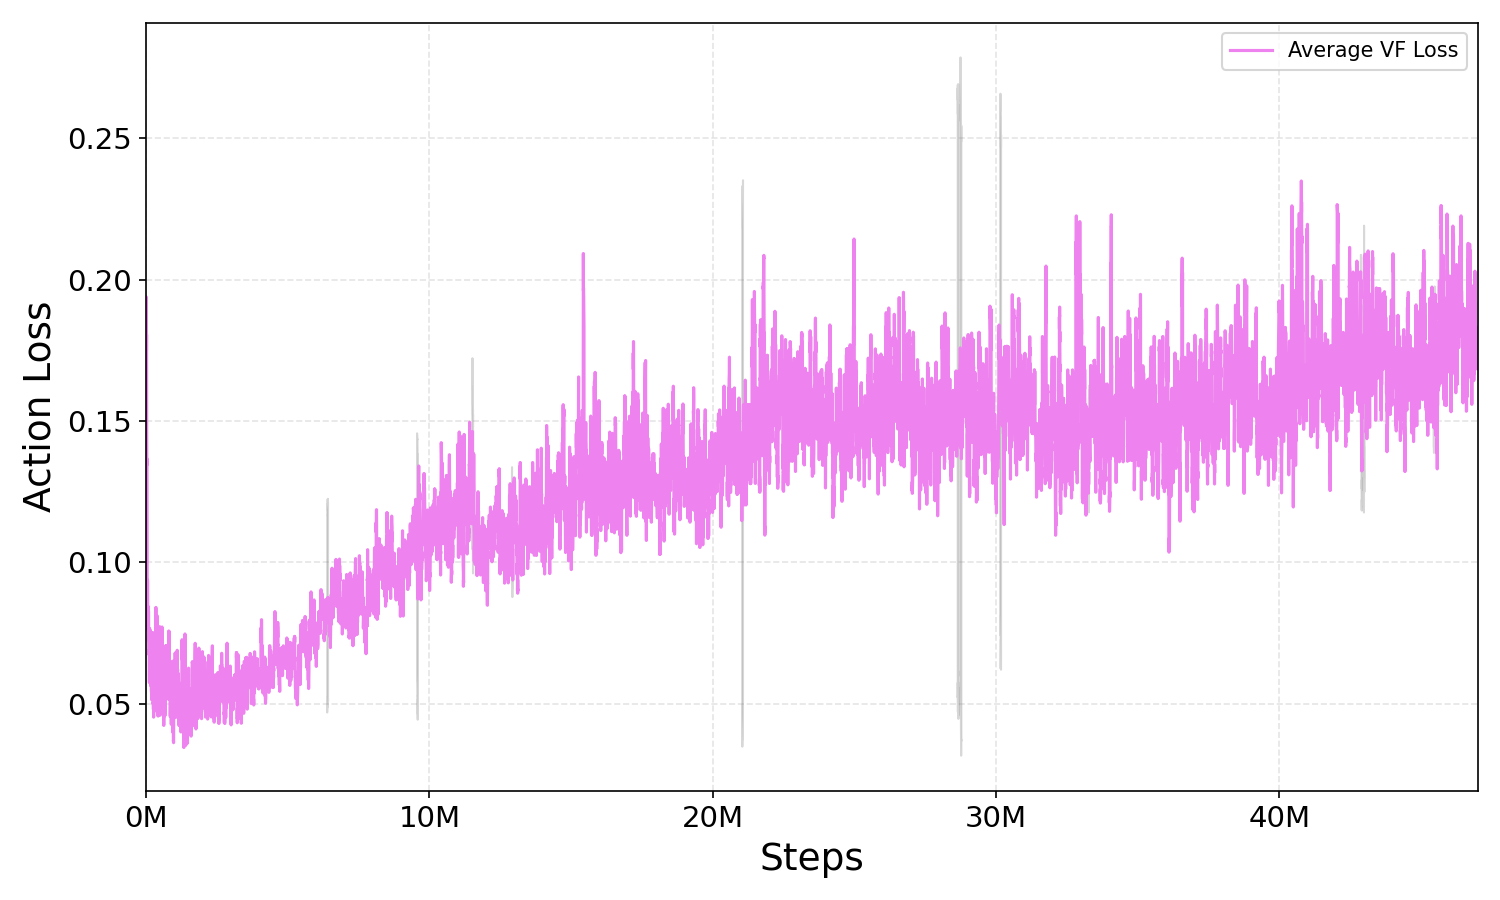
\includegraphics[width=\linewidth]{figures/offnav/offnav_losses_avg_std}
        \caption{OffNav average value function loss over four different runs.}
        \label{fig:training_problems_offnav}
    \end{subfigure}
    \hfill
    \begin{subfigure}[b]{0.49\linewidth}
        \centering
        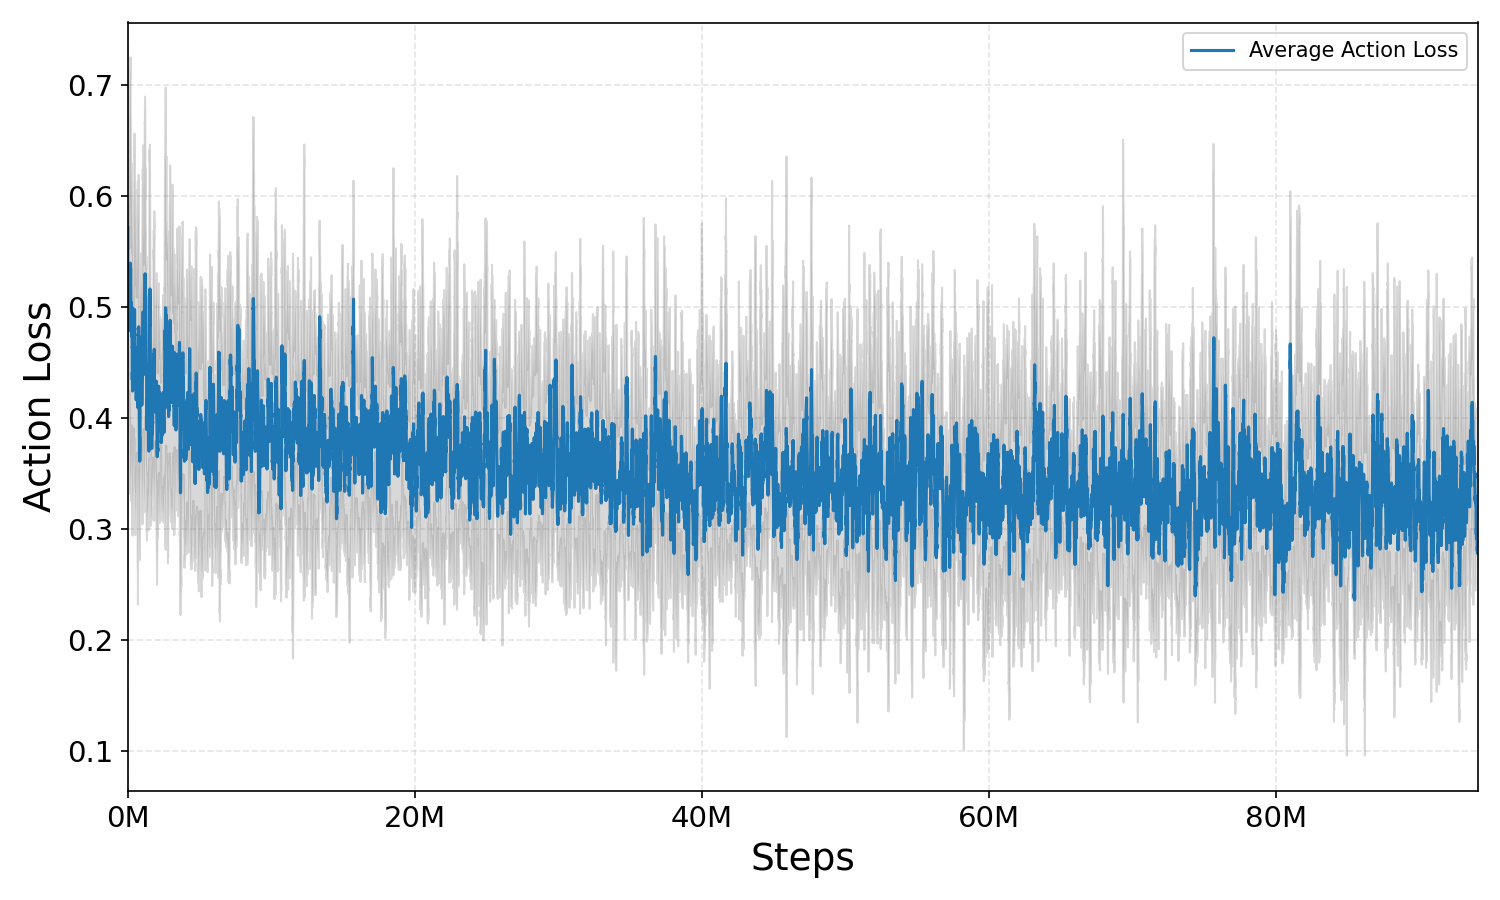
\includegraphics[width=\linewidth]{figures/metanav/metanav_losses_avg_std}
        \caption{MetaNav average action loss over four different runs.}
        \label{fig:training_problems_metanav}
    \end{subfigure}~\caption[Training curves of OffNav and Metanav]{Training curves of OffNav (\ref{fig:training_problems_offnav}) and Metanav (\ref{fig:training_problems_metanav}) on the full training dataset. The loss does not stabilize and even diverges, indicating the algorithm's inability to learn from the complete dataset.}
    \label{fig:training_problems}
\end{figure}

For these experiments, an extensive hyperparameter search was performed to find the best hyperparameters for each algorithm to achieve convergence.
Different pretrained initializations of the networks were also tested, but none of them were able to converge.
This suggests that the problem is not related to the hyperparameters or the initialization of the networks, but rather to the algorithms themselves.
Significant modifications to the baseline imitation learning algorithm~\cite{ramrakhya2023} or the baseline \acrshort{rl} algorithm~\cite{wijmans2020} like the ones presented in this chapter seem to hurt the performance of the trained agents when presented with a large dataset.

These last training efforts indicate that to go beyond the limitations of these algorithms, new approaches that do not modify substantially the underlying algorithm need to be explored.
For example, task inference methods~\cite{Beck_2025} could be a promising approach to tackle this problem.
These methods typically meta-train a context vector that summarizes the task information.
This context vector can then be used to condition the policy, allowing it to adapt to new tasks.
This approach could be compatible with more robust and proven algorithms like \acrshort{ddppo}~\cite{wijmans2020} or imitation learning~\cite{ramrakhya2023} that have proven to be effective in the past.